\documentclass[11pt]{article}

\usepackage[a4paper,margin=1in]{geometry}
\usepackage{graphicx}
\usepackage{booktabs}
\usepackage{array}
\usepackage{hyperref}
\usepackage{float}
\usepackage{xcolor}
\usepackage{enumitem}
\usepackage{titlesec}

\hypersetup{
  colorlinks=true,
  linkcolor=blue!50!black,
  urlcolor=blue!60!black
}

\titleformat{\section}{\large\bfseries}{\thesection}{0.7em}{}
\titleformat{\subsection}{\normalsize\bfseries}{\thesubsection}{0.6em}{}

\title{\textbf{Edge Detection in Noisy Images Using 2D Filtering}}
\author{ECE 0402 Group Project}
\date{\today}

\begin{document}

\maketitle

\section{Project Goal}
This project studies a narrow signals-and-systems question: why does naive edge detection fail in noisy images, and how can 2D filtering improve it? The project treats an image as a 2D signal and uses convolution, LTI filtering, derivative operators, and smoothing-before-detection as the main conceptual thread.

\section{Why This Topic Fits the Course}
\begin{itemize}[leftmargin=1.4em]
  \item The main system operation is 2D convolution.
  \item Sobel filtering is a direct example of a linear shift-invariant operator on a 2D signal.
  \item Edge detection highlights high-frequency structure, but noise also lives in that regime.
  \item The project includes a short demo that can be explained within two minutes.
\end{itemize}

\section{Method}
\subsection{Image Set}
The experiments use three standard images from \texttt{skimage.data} and one synthetic image generated in code. The synthetic image is useful because its geometry is fully controlled.

\begin{figure}[H]
  \centering
  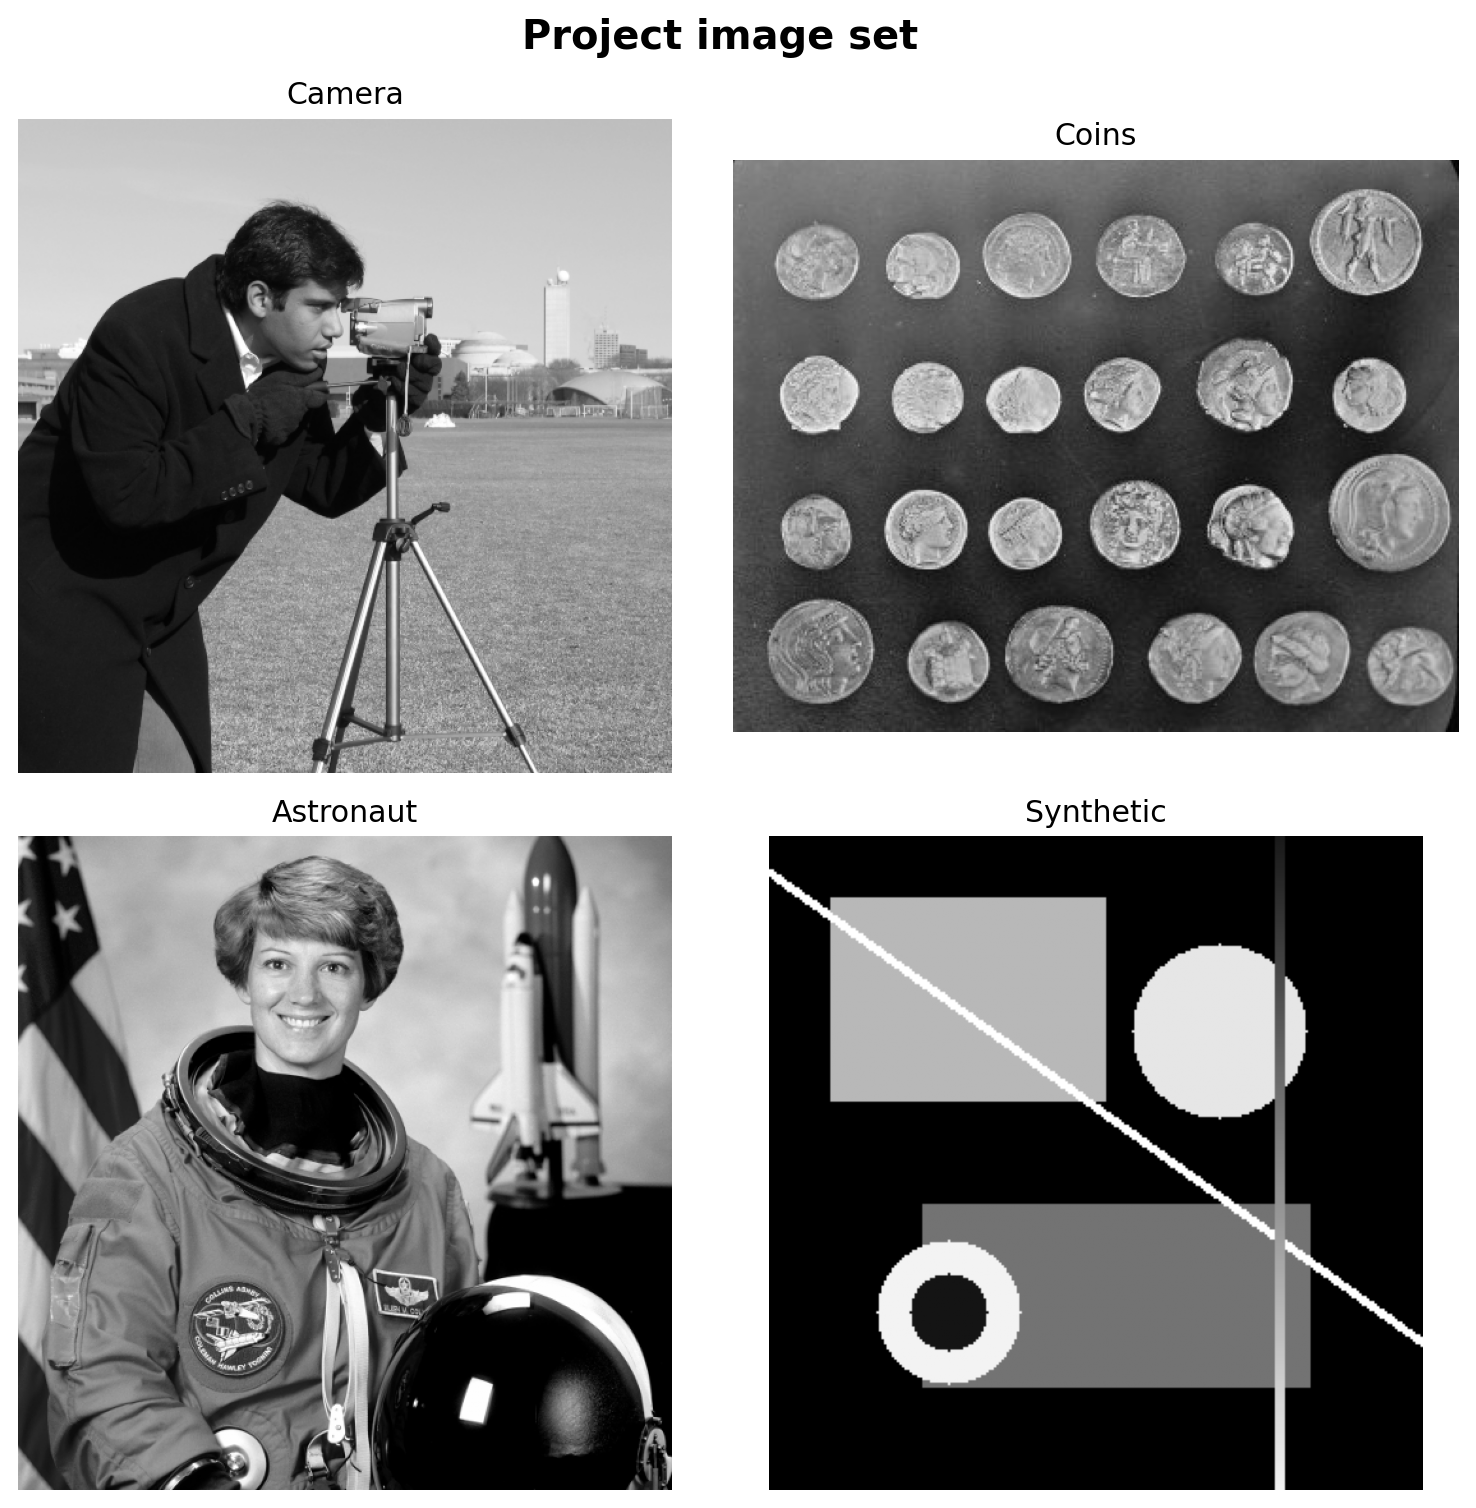
\includegraphics[width=0.72\linewidth]{../assets/generated/figures/image_gallery.png}
  \caption{Project image set used in the experiments.}
\end{figure}

\subsection{Pipeline}
The comparison pipeline is intentionally simple:
\begin{enumerate}[leftmargin=1.4em]
  \item apply Sobel directly to the clean image,
  \item add Gaussian noise and apply Sobel again,
  \item smooth the noisy image with a Gaussian filter before Sobel,
  \item compare the result with Canny as a stronger reference pipeline.
\end{enumerate}

The Sobel operator estimates horizontal and vertical intensity changes through two small convolution kernels.

\begin{figure}[H]
  \centering
  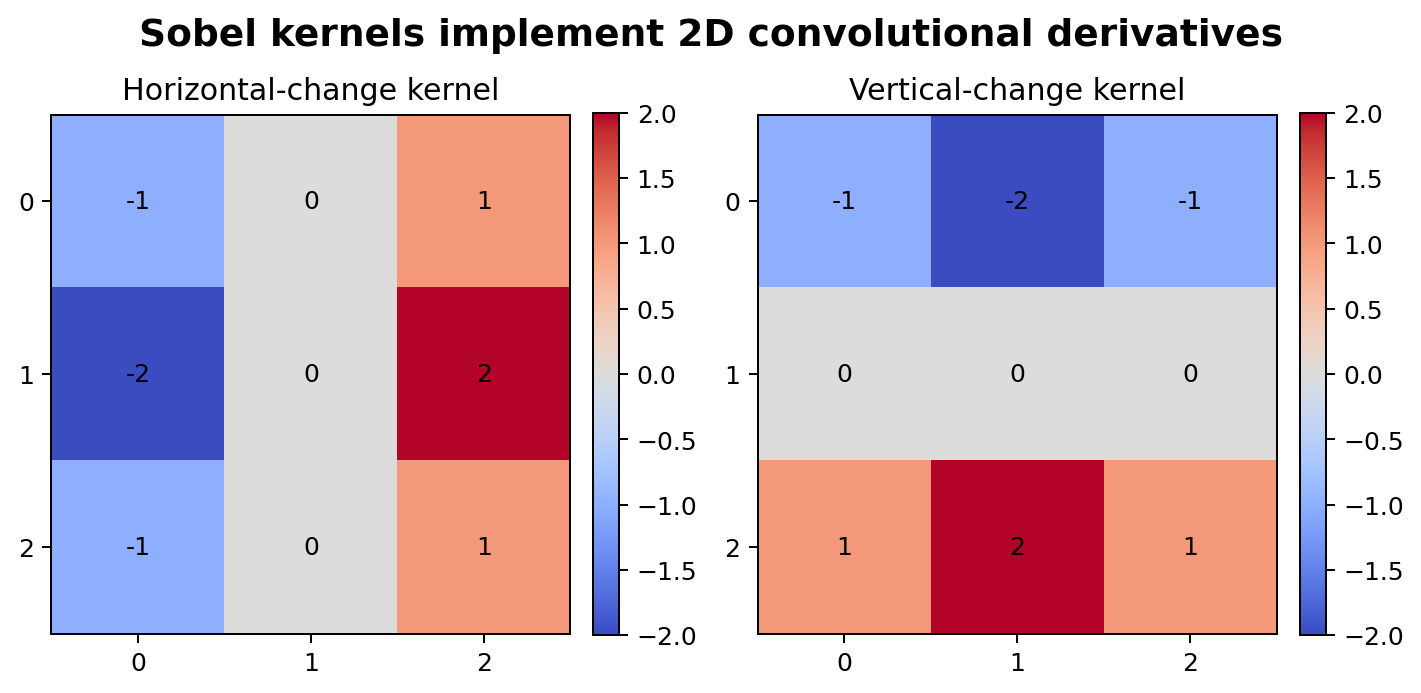
\includegraphics[width=0.62\linewidth]{../assets/generated/figures/sobel_kernels.png}
  \caption{Sobel kernels used to compute local derivatives in two dimensions.}
\end{figure}

\section{Key Result}
The core failure mode is easy to see: derivative filters amplify rapid changes, and noise is also a rapid change. This means naive edge detection reacts to random fluctuations as if they were meaningful boundaries.

\begin{figure}[H]
  \centering
  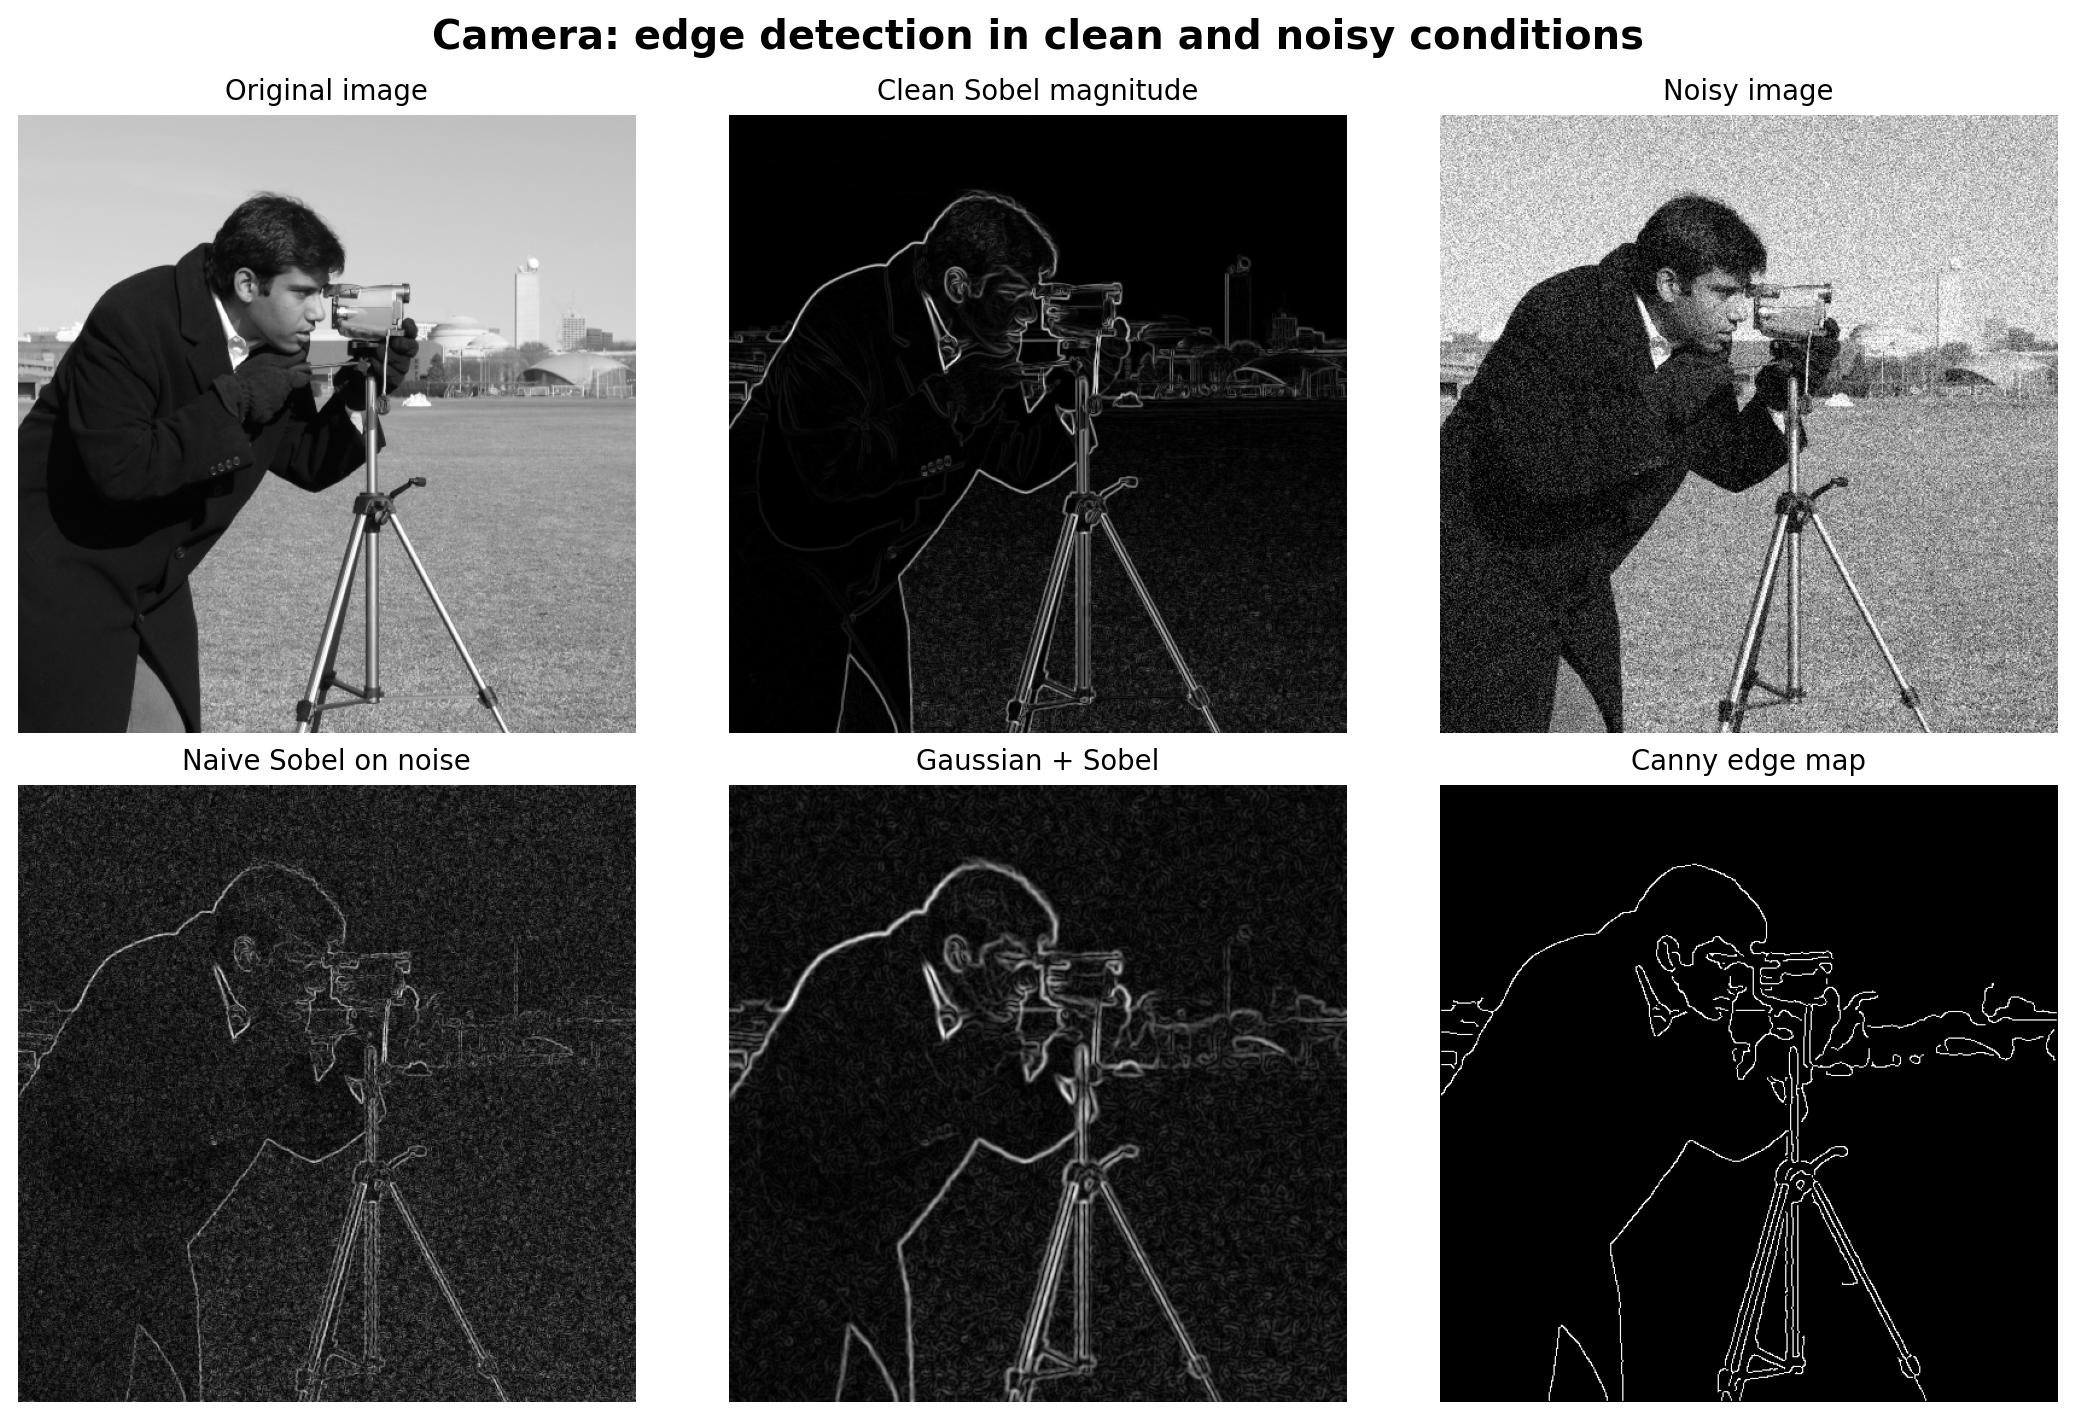
\includegraphics[width=\linewidth]{../assets/generated/figures/camera_pipeline.png}
  \caption{Main demo figure: noise corrupts the naive Sobel response, while smoothing and Canny improve the result.}
\end{figure}

\section{Tradeoff Analysis}
Smoothing helps, but too much smoothing weakens fine detail. To make that tradeoff explicit, the project computes an F1 score against a clean-edge reference over a grid of noise levels and smoothing strengths.

\begin{figure}[H]
  \centering
  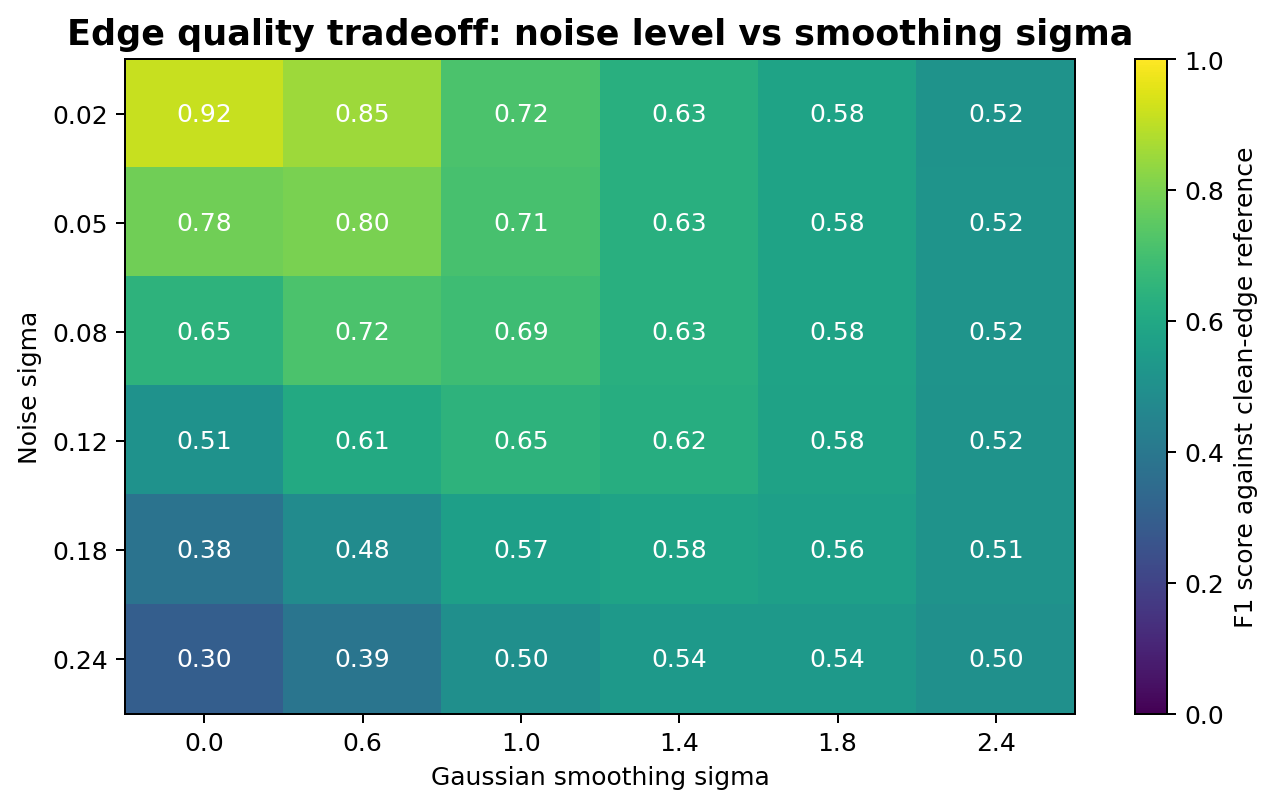
\includegraphics[width=0.74\linewidth]{../assets/generated/figures/tradeoff_heatmap.png}
  \caption{Tradeoff heatmap between noise level and smoothing strength.}
\end{figure}

The trend is straightforward:
\begin{itemize}[leftmargin=1.4em]
  \item when noise is small, little or no smoothing preserves the most detail;
  \item when noise increases, moderate smoothing improves edge quality;
  \item excessive smoothing eventually removes useful boundaries.
\end{itemize}

\section{Modern Vision Connection}
This project does not make CNNs or diffusion models the main story. That would be a category error. The point is to show that modern image models still rest on filtering intuition:
\begin{itemize}[leftmargin=1.4em]
  \item early CNN filters often learn edge-like or texture-like kernels;
  \item diffusion models repeatedly denoise an image estimate;
  \item classical filtering remains the correct conceptual baseline.
\end{itemize}

\section{Two-Minute Demo Script}
\begin{enumerate}[leftmargin=1.4em]
  \item Show the clean image and its Sobel response.
  \item Add Gaussian noise and show that naive Sobel now reacts to noise as if it were detail.
  \item Smooth the noisy image before Sobel and show the recovery of the main boundaries.
  \item End with Canny and explain why a better pipeline still depends on filtering.
\end{enumerate}

\section{Team Responsibilities Template}
Fill in the names before submission. Do not leave placeholder names in the final version.

\begin{table}[H]
  \centering
  \renewcommand{\arraystretch}{1.2}
  \begin{tabular}{p{0.18\linewidth} p{0.28\linewidth} p{0.38\linewidth}}
    \toprule
    Member & Responsibility & Concrete Output \\
    \midrule
    Member A & Project framing and literature check & Topic definition, references, slide story \\
    Member B & Implementation & Python modules, build script, generated figures \\
    Member C & Analysis and validation & Heatmap interpretation, self-check results, rehearsal timing \\
    Member D & Presentation assembly & Slide edits, speaking notes, final rehearsal \\
    \bottomrule
  \end{tabular}
  \caption{Template for explicit division of labor.}
\end{table}

\section{References}
\begin{enumerate}[leftmargin=1.4em]
  \item ECE 0402 course project guideline, \texttt{../Project Guideline\_ECE0402\_2026S.pdf}.
  \item scikit-image documentation, ``Canny edge detector,'' \url{https://scikit-image.org/docs/stable/auto_examples/edges/plot_canny.html}.
  \item scikit-image API documentation, \texttt{skimage.filters}, \url{https://scikit-image.org/docs/0.20.x/api/skimage.filters.html}.
  \item HIPR2, ``Sobel Edge Detector,'' \url{https://homepages.inf.ed.ac.uk/rbf/HIPR2/sobel.htm}.
  \item HIPR2, ``Canny Edge Detector,'' \url{https://homepages.inf.ed.ac.uk/rbf/HIPR2/canny.htm}.
  \item B. P. Lathi, \textit{Linear Systems and Signals}, 2nd edition.
  \item Luis F. Chaparro, \textit{Signals and Systems Using MATLAB}, 4th edition.
\end{enumerate}

\end{document}
